\chapter{Synchronization}
In concurrent programming where processes or threads cooperate and share data, race conditions may arise and there may be sections of not-reentrant code, it is needed to properly synchronize the cooperating actors to make their results not dependent on their relative speed.

A \emph{Critical Section} or \emph{Critical Region} is a section of code, common to multiple threads, in which they can access shared objects or in which they are competing for the use of shared resources. It is needed to ensure that when one thread is executing in its critical section, no other thread is allowed to execute in its critical section, therefore an access protocol must be established to enter the critical section in \textbf{mutual exclusion}:

\begin{itemize}
\item A thread executes a ``reservation'' code before entering a CS;
\item The reservation code blocks the thread if another is using its CS;
\item Leaving its CS, a thread executes a code to release the CS;
\item The release possibly unlocks another thread which was waiting in the ``reservation'' code of its CS.
\end{itemize}

In general, the \textbf{software solutions} to the problem of CS are complex and inefficient. In fact, test and set operations are ``invisible'' to the other threads and they are not atomic, thus a thread can react to the presumed value of a variable rather than to its current value. Furthermore, the solutions is not easily extensible to an arbitrary number of threads.

The \textbf{hardware solutions} can be easily extensible to a larger number of threads but they introduce busy form of waiting with spin lock leading to possible starvation.

\section{Semaphores}
The hardware solution can be used to implement system calls that can be used for solving every kind of synchronization problem (not only the Mutual Exclusion) avoiding the busy form of waiting. These system calls rely on a data structure introduce by Dijkstra in 1965 called semaphore.

A \emph{semaphore} is a shared structure including a counter, a waiting queue managed by the kernel both protected by a lock.
The kernel offers a set of \textbf{atomic primitives} that allows a thread to be blocked on the semaphore or to wake up if it was locked.

\begin{description}
\item \texttt{init(S, k)} defines and initializes semaphore \texttt{S} counter to value \texttt{k}. \texttt{k} is a positive value because the system calls manage the counter so that, if negative, its absolute value is the number of threads waiting on the semaphore queue.
\item \texttt{wait(S)} decrements the counter and blocks the calling thread if the counter value of \texttt{S} is negative or zero.
\item \texttt{signal(S)} increases the counter and made some blocked threads ready to run if the counter value of \texttt{S} is negative or zero.
\item \texttt{destroy(S)} releases semaphore \texttt{S} memory.
\end{description}

Semaphores can be used to solve any synchronization problem using an appropriate protocol, possibly adding more than one semaphore and additional share variables.

\subsection{POSIX semaphores}
POSIX semaphores define a set of kernel independent system calls, included in header file \texttt{semaphore.h} which return -1 on error.

\begin{description}
\item \texttt{int sem\_init(sem\_t *sem, int pshared, usigned int value)} initializes the semaphore counter at value \texttt{value}. The \texttt{pshared} value identifies the type of semaphore. If it is equal to 0, the semaphore is local to the threads of current process, otherwise the semaphore can be shared between different processes.

\item \texttt{int sem\_wait(sem\_t *sem)} implements the standard wait, i.e.\@ if the counter is negative or zero, the calling thread is blocked.

\item \texttt{int sem\_post(sem\_t *sem)} implements the standard signal, i.e.\@ increments the counter and wakes up a blocking thread if the counter is negative or zero.

\item \texttt{int sem\_getvalue(sem\_t *sem, int *valP)} allows obtaining the value of the semaphore counter. The value is assigned to \texttt{*valP}.

\item \texttt{int sem\_destroy(sem\_t *sem)} destroys the semaphore at the address pointed by \texttt{sem}.

\item \texttt{int sem\_trywait(sem\_t *sem)} implements a non-blocking wait, i.e.\@ if the semaphore counter has a value greater than 0, it performs the decrement and returns 0 while, if the semaphore counter is negative or zero, it returns -1 instead of blocking the caller as \texttt{sem\_wait} does.
\end{description}

\subsection{Pthread mutex}
Pthread mutex defines binary semaphores of type \texttt{pthread\_mutex\_t} by means of system calls
\begin{description}
\item \texttt{int pthread\_mutex\_init(pthread\_mutex\_t *mutex, \newline const pthread\_mutexattr\_t *attr)} initializes the mutex referenced by \texttt{mutex} with attributes specified by \texttt{attr} (default = \texttt{NULL}).

\item \texttt{int pthread\_mutex\_lock(pthread\_mutex\_t *mutex)} blocks the caller if the \texttt{mutex} is locked or acquires the mutex lock if the \texttt{mutex} is unlocked.

\item \texttt{int pthread\_mutex\_trylock(pthread\_mutex\_t *mutex)} is similar to a \texttt{lock}, but returns without blocking the caller if \texttt{mutex} is locked. It returns 0 if the lock has been successfully acquired or a \texttt{EBUSY} error if  the \texttt{mutex} was already locked.

\item \texttt{int pthread\_mutex\_unlock(pthread\_mutex\_t *mutex)} releases the \texttt{mutex} lock.

\item \texttt{int pthread\_mutex\_destroy(pthread\_mutex\_t *mutex)} frees \texttt{mutex} memory so that it cannot be used anymore.
\end{description}

\section{Synchronization protocols with semaphores}
\subsection{Producer \& Consumer with limited memory buffer}
This problem uses a circular buffer implementing a FIFO queue of size \texttt{MAX} for storing the produced elements to be consumed. If the buffer is empty, the consumer has to wait. On the other hand, if the buffer is full, the producer has to wait. In an intermediate situation, producer and consumer can produce and consume in a concurrent fashion.

\begin{figure}[hbtp]
\centering
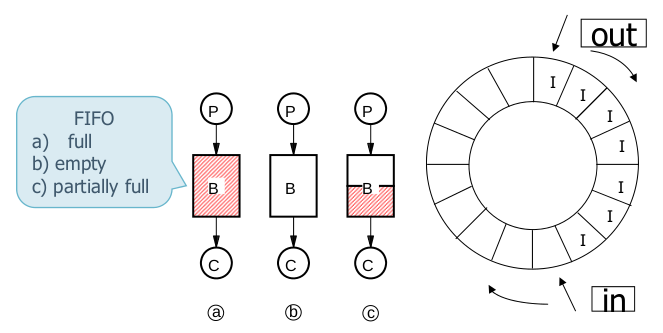
\includegraphics[scale=0.4]{images/synchronization/producer_consumer_buffer.png}
\caption{Circular buffer}
\end{figure}

\paragraph{Access functions}
Functions without considering synchronization and concurrency.
\begin{Parallel}{}{}
\ParallelLText{
\begin{verbatim}
void enqueue(int val) {
  queue[in] = val;
  in = (in + 1) % MAX;
  return;
}
\end{verbatim}}
\ParallelRText{
\begin{verbatim}
void dequeue(int *val) {
  queue[out] = val;
  out = (out + 1) % MAX;
  return;
}
\end{verbatim}}
\end{Parallel}

\paragraph{Concurrent access}
Initially, a consumer has to wait and a producer has to produce, i.e.\@ it has not to be blocked. Therefore, a consumer has to wait on full, initialized to 0 and a producer has to produce at most \texttt{MAX} elements. Both signal when an elements is enqueued or dequeued.
\begin{verbatim}
init(full, 0);
init(empty, MAX);
\end{verbatim}

\begin{Parallel}{}{}
\ParallelLText{
\begin{verbatim}
Producer() {
  Message m;
  while(TRUE) {
    produce(m);
    wait(empty);
    enqueue(m);
    signal(full);
  }
}
\end{verbatim}}
\ParallelRText{
\begin{verbatim}
Consumer() {
  Message m;
  while(TRUE) {
    wait(full);
    m = dequeue();
    signal(empty);
    consume(m);
  }
}
\end{verbatim}}
\end{Parallel}

Producer and consumer operate on different indexes of the buffer, thus they can operate in concurrency as long as the queue is not full or empty, otherwise either a producer or a consumer is blocked.

The solution is symmetric and it can be easily extended to more than one producer and consumer processes, remembering that operations on the queue are not atomic and multiple consumers or multiple producers must act in mutual exclusion.

\paragraph{Producers \& Consumers}
\begin{verbatim}
init(full, 0);
init(empty, MAX);
init(meP, 1);
init(meC, 1);
\end{verbatim}

\begin{Parallel}{}{}
\ParallelLText{
\begin{verbatim}
Producer() {
  Message m;
  while(TRUE) {
    produce(m);
    wait(empty);
    wait(meP);
    enqueue(m);
    signal(meP);
    signal(full);
  }
}
\end{verbatim}}
\ParallelRText{
\begin{verbatim}
Consumer() {
  Message m;
  while(TRUE) {
    wait(full);
    wait(meC);
    m = dequeue();
    signal(meC);
    signal(empty);
    consume(m);
  }
}
\end{verbatim}}
\end{Parallel}

\newpage

\subsection{Readers \& Writers}
This represents the typical problem of sharing a database between two sets of concurrent threads:
\begin{itemize}
\item Readers are allowed to access the database in concurrency;
\item Writers must access the database in Mutual Exclusion with other Writers and Readers.
\end{itemize}
When a writer is writing in the database, several Readers and Writers processes can be blocked waiting the end of the write operation.

\textbf{Readers precedence}: at the end of a writing operation, favour the access of the waiting Readers rather than of the waiting Writers.

\textbf{Writers precedence}: at the end of a writing operation, favour the access of the waiting Writers rather than of the waiting Readers.

\paragraph{Readers priority}
Giving priority to the Readers means that a Reader does not wait unless a Writer is writing.

While Readers are reading, new Readers are allowed to read and Writers are blocked. The first Reader blocks any Writer and, dually, when the last Reader terminates, a waiting Writer can access the database.

The solution uses:
\begin{itemize}
\item A shared variable \texttt{nR} that counts the number of Readers inside the critical section;
\item A Mutual Exclusion semaphore \texttt{meR} to protect variable \texttt{nR};
\item A Mutual Exclusion semaphore \texttt{w} among Writers or among Readers and Writers;
\item A Mutual Exclusion semaphore \texttt{meW} among Writers.
\end{itemize}

\begin{verbatim}
nR = 0;
init(meR, 1);
init(meW, 1);
init(w, 1);
\end{verbatim}

\begin{Parallel}{}{}
\ParallelLText{
\begin{verbatim}
Reader() {
  wait(meR);
    nR++;
    if(nR == 1)
      wait(w);
  signal(meR);
  // read
  wait(meR);
    nR--;
    if(nR == 0)
      signal(w);
  signal(meR);
}
\end{verbatim}}
\ParallelRText{
\begin{verbatim}
Writer() {
  wait(meW);
  wait(w);
  // write
  signal(w);
  signal(meW);
}
\end{verbatim}}
\end{Parallel}

\paragraph{Writers priority}
Giving priority to the Writers means that a Writer has priority over all Readers.

A Writer trying to enter its critical section blocks \emph{new} Readers, but the Readers that are inside their critical section are allowed to complete their reading task.

The solution uses:
\begin{itemize}
\item Two shared variables \texttt{nR} and \texttt{nW} to count the Readers inside the critical section and the Writers that need to write (one of them possibly writing);
\item Two Mutual Exclusion semaphores \texttt{meR} and \texttt{meW} to protect the variables \texttt{nR} and \texttt{nW};
\item Two Mutual Exclusion semaphores \texttt{r} and \texttt{w} to enforce Readers and Writers to wait on different queues.
\end{itemize}

\begin{verbatim}
nR = nW = 0;
init(meR, 1);
init(meW, 1);
init(w, 1);
init(r, 1);
\end{verbatim}

\begin{Parallel}{}{}
\ParallelLText{
\begin{verbatim}
Reader() {
  wait(r);
    wait(meR);
      nR++;
      if(nR == 1)
        wait(w);
    signal(meR);
  signal(r);
  // read
  wait(meR);
    nR--;
    if(nR == 0)
      signal(w);
  signal(meR);
}
\end{verbatim}}
\ParallelRText{
\begin{verbatim}
Writer() {
  wait(meW);
    nW++;
    if(nW == 1)
      wait(r);
  signal(meW);
  wait(w);
  // write
  signal(w);
  wait(meW);
    nW--;
    if(nW == 0)
      signal(r);
  signal(meW);
}
\end{verbatim}}
\end{Parallel}

\subsection{Single lane tunnel}
A tunnel has a single lane, and cars can proceed only in alternate directions. Therefore it is needed to enable any number of cars (threads) to proceed in the same direction and block traffic in one direction if there is traffic in the opposite one.

\begin{figure}[hbtp]
\centering
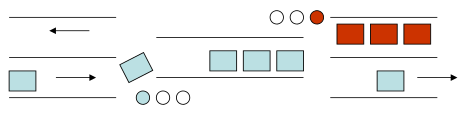
\includegraphics[scale=0.4]{images/synchronization/single_lane_tunnel.png}
\caption{Single lane tunnel}
\end{figure}


This problem is similar the Readers \& Writers one, but for two sets of Readers. In its basic implementation can result in starvation of cars in one direction.

The solution uses:
\begin{itemize}
\item Two shared count variables \texttt{n1} and \texttt{n2}, one for each travel direction;
\item Two semaphores \texttt{s1} and \texttt{s2}, one for each travel direction;
\item A global semaphore wait \texttt{busy}.
\end{itemize}

\begin{verbatim}
n1 = n2 = 0;
init(s1, 1);
init(s2, 1);
init(busy, 1);
\end{verbatim}

\begin{Parallel}{}{}
\ParallelLText{
\begin{verbatim}
left2right() {
  wait(s1);
    n1++;
    if(n1 == 1)
      wait(busy);
  signal(s1);
  // run left to right
  wait(s1);
    n1--;
    if(n1 == 0)
      signal(busy);
  signal(s1);
}
\end{verbatim}}
\ParallelRText{
\begin{verbatim}
right2left() {
  wait(s2);
    n2++;
    if(n2 == 1)
      wait(busy);
  signal(s2);
  // run right to left
  wait(s2);
    n2--;
    if(n" == 0)
      signal(busy);
  signal(s2);
}
\end{verbatim}}
\end{Parallel}

\subsection{Conditions}
A \emph{condition} is a data structure containing a mutual exclusion lock, a condition variable and a data structure to protect because it require synchronization.

\begin{verbatim}
typedef struct Cond {
  pthread_mutex_t lock;
  pthread_cond_t mycond;
  int i;
} Cond;
\end{verbatim}

\begin{description}
\item \texttt{lock} protects the structure;
\item \texttt{mycond} is the condition variable;
\item \texttt{i} is the variable to set or check.
\end{description}

Main thread has to define such a structure, allocate a global structure of that type, initialize its variables and create two threads A and B.

Thread A does work until it needs to check a given condition by calling \texttt{pthread\_cond\_wait} to wait for a signal from thread B, unlocking the lock (otherwise, no one can change the variable content). When signaled, thread A wakes up with lock locked and, after explicitly unlocking the lock, can continues its work.

Thread B does work and locks the condition lock. It changes the value of the global variable associated to the waiting condition and, if thread A wait condition is true, it performs a \texttt{pthread\_cond\_signal}. After unlocking the condition lock, it can continue its work.

\paragraph{Waiting on Condition Variables}
\begin{description}
\item \texttt{int pthread\_cond\_wait(pthread\_cond\_t *cond, \newline pthread\_mutex\_t *mutex)} blocks the calling thread until the specified condition is signaled. This system call should be called while \textit{lock} is locked, and it will automatically release the \textit{lock} while it waits.

After signal is received and thread is awakened, lock be automatically locked for use by the thread.

The programmer is then responsible for unlocking lock when the thread does not more need it.
\end{description}

\paragraph{Signaling on Condition Variables}
\begin{description}
\item \texttt{int pthread\_cond\_signal(pthread\_cond\_t *cond)} signals another thread which is waiting on the condition variable.

It should be called with the \textit{lock} locked, and must unlock the \textit{lock} to allow \texttt{pthread\_cond\_wait} to complete.

\item \texttt{int pthread\_cond\_broadcast(pthread\_cond\_t *cond)} \newline
should be used if more than one thread is blocked on the same condition variable, rather than \texttt{pthread\_cond\_signal}. It is a logical error to call \texttt{pthread\_cond\_signal} before calling \texttt{pthread\_cond\_wait}.
\end{description}

\subsection{Precedence graphs}
Goal is to implement a graph using the minimum number of semaphores remembering that signals are sent to a semaphore, not to a process and they are caught by the first process able to receive them.

The first thing to do is to delete arcs which are not necessary and can, therefore, lead to use a non minimum number of semaphores.

\textbf{Acyclic threads}: outgoing arcs require a single semaphore and incoming arcs require a single semaphore.

\textbf{Cyclic threads}: outgoing arcs require different semaphores, while incoming arcs use a single  semaphore. In fact, using the same semaphore, because of the loop statement, a single process can get two signals if it is very fast.